\documentclass[aps,prl,twocolumn,showpacs,superscriptaddress,groupedaddress,nofootinbib,floatfix]{revtex4}  % for review and submission
%\documentclass[aps,preprint,showpacs,superscriptaddress,groupedaddress]{revtex4}  % for double-spaced preprint
\usepackage{graphicx}  % needed for figures
\usepackage{dcolumn}   % needed for some tables
\usepackage{bm}        % for math
\usepackage{amsmath,amssymb}   % for math
\usepackage{aas_macros}
\usepackage{multirow}
\usepackage{color}
\usepackage{verbatim}
\usepackage{times}
\usepackage{url}
\usepackage{hyperref}

% avoids incorrect hyphenation, added Nov/08 by SSR
\hyphenation{ALPGEN}
\hyphenation{EVTGEN}
\hyphenation{PYTHIA}

\newcommand{\mr}{\mathrm}
\newcommand{\tcb}{\textcolor{blue}}


\begin{document}
% The following information is for internal review, please remove them for submission
\widetext
% the following line is for submission, including submission to the arXiv!!
%\hspace{5.2in} \mbox{Fermilab-Pub-04/xxx-E}

\title{Recovering Lost 21cm Radial Modes via Cosmic Tidal Reconstruction}

\author{Hong-Ming Zhu}
\affiliation{Key Laboratory for Computational Astrophysics, National Astronomical Observatories, Chinese Academy of Sciences, 20A Datun Road, Beijing 100012, China}
\affiliation{University of Chinese Academy of Sciences, Beijing 100049, China}

\author{Ue-Li Pen} 
\affiliation{Canadian Institute for Theoretical Astrophysics, University of Toronto, 60 St. George Street, Toronto, Ontario M5S 3H8, Canada}
\affiliation{Dunlap Institute for Astronomy and Astrophysics, University of Toronto, 50 St. George Street, Toronto, Ontario M5S 3H4, Canada}
\affiliation{Canadian Institute for Advanced Research, CIFAR Program in Gravitation and Cosmology, Toronto, Ontario M5G 1Z8, Canada}
\affiliation{Perimeter Institute for Theoretical Physics, 31 Caroline Street North, Waterloo, Ontario, N2L 2Y5, Canada}

\author{Yu Yu}
\affiliation{Key Laboratory for Research in Galaxies and Cosmology,
Shanghai Astronomical Observatory, Chinese Academy of Sciences,
80 Nandan Road, Shanghai 200030, China}

\author{Xuelei Chen}
\affiliation{Key Laboratory for Computational Astrophysics,  National Astronomical Observatories, Chinese Academy of Sciences, 20A Datun Road, Beijing 100012, China}
\affiliation{University of Chinese Academy of Sciences, Beijing 100049, China}
\affiliation{Center of High Energy Physics, Peking University, Beijing 100871, China}
\date{\today}

\begin{abstract}
21 cm intensity mapping has emerged as a promising technique to map the 
large-scale structure of the Universe, at redshifts $z$ from 1 to 10.
Unfortunately, many of the key cross correlations with photo-$z$ galaxies
and the CMB have been thought to be impossible due to foreground
contamination for radial modes with small wavenumbers. 
These modes are usually subtracted in the foreground subtraction process.
We recover the lost 21 cm radial modes via cosmic tidal reconstruction and 
find more than 60\% cross-correlation signal at $\ell\lesssim100$ and 
even more on larger scales can be recovered from null. 
The tidal reconstruction method opens up a new set of possibilities to 
probe our Universe and is extremely valuable not only for 21 cm surveys
but also for CMB and photometric redshift observations.
\end{abstract}

\pacs{}
\maketitle

%\section{\label{sec:level1}First-level heading}
% sections are not used for PRL papers

{\it Introduction.}---The current and future cosmological observations aim
to map a large fraction of the Universe with unprecedent precision, varying
from LSST \cite{2009:lsst}, Euclid \cite{2012:euclid}, 
Planck \cite{2015arXiv150201582P}, CMB-S4 \cite{2014ApJ...788..138W}, and etc. 
In addition to these ones, 21 cm intensity mapping has emerged as
a powerful probe of the 
cosmological large-scale structure \cite{2008:21cm,chang}.
However, the astrophysical foregrounds from galactic and extra-galactic
synchrotron and free-free emissions are stronger than the cosmological 21 cm 
signals by many orders of magnitude. These foregrounds are expected to be 
spectrally smooth, which means they would contaminate small radial
modes, i.e., all modes with low $k_\parallel$.
While there are not many modes with small $k_\parallel$, many other cosmic
observations with broad window functions along the radial direction only 
probe these modes, such as weak lensing, photo-$z$ galaxies, 
integrated Sachs-Wolf effect, kinetic Sunyaev-Zel'dovich effect, and etc.  
Thus, 
%this makes it very hard to cross correlate these cosmic probes with 
%21 cm intensity mapping surveys 
the cross correlations of 21 cm surveys with these cosmic probes are dominated 
by foreground contamination \cite{2007ApJ...660.1030F,2008MNRAS.384..291A}. 
To solve this problem is of great importance for both 21 cm 
intensity mapping surveys and other key cosmic surveys.

Recently a new method called {\it cosmic tidal reconstruction} has been 
developed \cite{2012:pen,2015:zhu}. It can reconstruct the large-scale 
tidal field and hence large-scale density field from the alignment of 
small-scale cosmic structures.
The modes with small $k_\parallel$ and large $k_\perp$ are well 
reconstructed \cite{2015:zhu}, which are exactly those lost in the foreground 
subtraction in 21 cm experiments. 
This technique enables the reconstruction of small radial modes, 
which provides important radial information essential for cross correlating 
with CMB and other cosmic probes.

%which are essential for CMB and other cross correlations.

In this Letter we study how to use cosmic tidal reconstruction to 
reconstruct the lost large-scale radial modes, and further cross correlate with
CMB lensing, photo-$z$ galaxies and ISW effect. 
We find such reconstruction technique recovers more than 60\% cross-correlation 
signal at $\ell\lesssim100$ from nothing and even better on larger scales. 
This provides a new way to probe the origin and evolution of the Universe.

{\it Cosmic tidal reconstruction.}---Cosmic tides is a new way to view the
tidal effect of gravity on the structure of matter clustering \cite{2012:pen}.
The large-scale density field can be reconstructed accurately from the 
anisotropic tidal distortions of the locally-measured matter power spectrum
\cite{2012:pen,2015:zhu}.
The basic idea of purely transverse tidal reconstruction has been proposed in
Ref. \cite{2012:pen} and further expanded in Ref. \cite{2015:zhu}.
Here, we briefly discuss the idea and summarize the process of cosmic
tidal reconstruction. 

The evolution of small-scale density perturbations is modulated by 
long-wavelength perturbations \cite{2014:tidal}. 
The anisotropic distortions in the local small-scale matter power specturm,
$\propto\hat{k}^i\hat{k}^jt_{ij}^{(0)}$, arise from the coupling of small-scale
density fluctuations with the large-scale tidal field $t_{ij}$, where 
$t_{ij}=\Phi_{L,ij}-\delta_{ij}\nabla^2\Phi_L/3$, $\hat{\ }$ denotes the 
unit vector and superscript (0) denotes some ``initial'' time. 
The traceless tidal field $t_{ij}$ can be decomposed into 5 independently 
observable components \cite{2015:zhu}.
The two transverse shear terms, 
$\gamma_1=(\Phi_{L,11}-\Phi_{L,22})/2$ and $\gamma_2=\Phi_{L,12}$,
which describe quadrupolar distortions in the tangential plane perpendicular
to the line of sight, are less affected by peculiar velocities and used to 
perform reconstruction \cite{2015:zhu}.
%Since 
%Here, $\gamma_1=(\Phi_{L,11}-\Phi_{L,22})/2$ and $\gamma_2=\Phi_{L,12}$
%only involves derivatives in the tangential plane, the changes in $\gamma_1$
%and $\gamma_2$ due to the redshift space distortions are expected to be second
%order effects. 
The two gravitational tidal shear fields $\gamma_1$ and $\gamma_2$
can be converted to the two-dimensional (2D) convergence field, 
$\kappa_\mr{2D}=(\Phi_{L,11}+\Phi_{L,22})/2$, using
\begin{eqnarray}
\label{eq:kappa2d}
\kappa_{\mr{2D},11}+\kappa_{\mr{2D},22}=
(\gamma_{1,11}-\gamma_{1,22}+2\gamma_{2,12}).
\end{eqnarray}
The three-dimensional (3D) convergence $\kappa_\mr{3D}=\nabla^2\Phi_L/3\propto\delta_L$, which gives
the large-scale density field, is given by 
\begin{eqnarray}
\label{eq:kappa3d}
\kappa_{\mr{3D},11}+\kappa_{\mr{3D},22}=\frac{2}{3}\nabla^2\kappa_\mr{2D}.
\end{eqnarray}
Since only two transverse tidal shear fields $\gamma_1(\bm{x})$ and 
$\gamma_2(\bm{x})$ are used, the changes of the large-scale density field along
the line of sight are inferred from the variations of $\gamma_1$ and $\gamma_2$
along the $x_\parallel$ axis. The error of $\kappa_\mr{3D}$ is 
\begin{eqnarray}
\sigma_{\kappa_\mr{3D}}(\bm{k})\propto\big({k^2}/{k_\perp^2}\big)^2,
\end{eqnarray}
which is anisotropic in $k_\perp$ and $k_\parallel$ \cite{2015:zhu}.
The reconstruction works best for modes with low $k_\parallel$ and high 
$k_\perp$, which can not be obtained from 21 cm surveys and contribute 
substantially to cosmological observables from other surveys mentioned above.
Thus, cosmic tidal reconstruction provides a new way to recover the lost 
radial modes and to improve the cross correlations.

The tidal reconstrction works as follows. The first step is to convolve
the density field with a Gaussian kernel, $S(\bm{k})=e^{-k^2R^2/2}$, which
filters out the small-scale nonlinear structures.
Here, we still take $R=1.25\ \mr{Mpc}/h$ \cite{2012:pen,2015:zhu}. The
next step is to gaussianize the smoothed density field by taking a logarithmic
transform or mapping the density fluctuations into a Gaussian distribution. 
In the following reconstructions, we adopt the latter method since after the
simulated
foreground subtraction, some of the density contrasts become smaller than $-1$,
which makes it hard to take the logarithmic transform, $\mathrm{ln}(1+\delta)$.
The gravitational tidal shear fields can be estimated by applying quadratic 
tidal shear estimators $\hat{\gamma}_1$ and $\hat{\gamma}_2$ to the density 
field as in 21 cm lensing reconstruction \cite{2008:lu}. 
Then the 3D tidal convergence field $\kappa_\mr{3D}$ is given by the linear 
combination of tidal shear fields using Eq. (\ref{eq:kappa2d}) and 
Eq. (\ref{eq:kappa3d}).
The reconstructed noisy field $\kappa_\mr{3D}$ is related to the original 
density field as 
\begin{eqnarray}
\kappa_\mr{3D}(k_\perp,k_\parallel)=b(k_\perp,k_\parallel)
\delta(k_\perp,k_\parallel)+n(k_\perp,k_\parallel),
\end{eqnarray}
where $b=P_{\kappa_\mr{3D}\delta}/P_{\delta}$ is the bias factor and $n$ is 
the noise of reconstruction \cite{2015:zhu}. 
The reconstructed clean field is given by 
\begin{eqnarray}
\label{eq:kapc}
\hat{\kappa}_c=({\kappa_\mr{3D}}/{b})W,
\end{eqnarray}
where the Wiener filter $W(k_\perp,k_\parallel)=
P_\delta/(P_{\kappa_\mr{3d}}/b^2)$.

{\it Simulation setup.}---We further explore this idea with numerical 
simulations. We employ an ensemble of six $N$-body simulations from the
$\mr{CUBEP}^3\mr{M}$ code \cite{2013:code}. 
Each simulation includes $1024^3$ particles in a $(1.2\mr{Gpc}/h)^3$ box. 
%with following cosmological parameters: Hubble parameter $h=0.678$, baryon
%density $\Omega_{b}=0.049$, dark matter density $\Omega_{c}=0.259$,
%amplitude of primordial curvature power spectrum $A_s=2.139\times10^{-9}$ at 
%$k_0=0.05\;\mr{Mpc}^{-1}$ and scalar spectral index $n_s=0.968$.
In the following analysis we use outputs at $z=1$.

\begin{figure}[tbp]
\begin{center}
\includegraphics[width=0.48\textwidth]{1.000cc2d.eps}
\end{center}
\vspace{-0.7cm}
\caption{(Top) The cross-correlation coefficient of the  
foreground subtracted density field with the original density field.
%$r_{\delta_{fs}\delta}=P_{\delta_{fs}\delta}/\sqrt{P_{\delta_{fs}}P_\delta}$. 
(Bottom) The cross-correlation coefficient of the reconstructed field with 
the original density field. 
%$r_{\kappa_{c}\delta}=P_{\kappa_{c}\delta}/\sqrt{P_{\kappa_{c}}P_\delta}$. 
The lost radial modes appear again after reconstruction.
The results are for $R_\parallel=60\ \mr{Mpc}/h$ and $k_c=0.5\ h/\mr{Mpc}$.}
\label{fig:ratio}
\end{figure}

We could approximately use dark matter to represent 21 cm source distributions.
This is a good approximation since the neutral hydrogen traces the total mass
distribution fairly well at low redshifts. We simply assume the experimental
noise to be zero above a cut off scale and infinity below the cut off scale.
This is a reasonable approximation for a filled aperture experiment, which
has good brightness sensitivity and an exponetially growing noise at small 
scales.
We choose this scale to be $k_c=0.5\ h/\mr{Mpc}$, which corresponds to 
$\ell=1150$ at $z=1$. This is realistic for the ongoing 21 cm experiments like
CHIME \cite{2014SPIE.9145E..22B}, Tianlai \cite{2015ApJ...798...40X}, 
HIRAX \cite{HIRAX}, and etc.

We are not going to provide a detailed 21 cm data reduction process in this 
Letter, so we simply  use a high-pass filter 
$W_{fs}(k_\parallel)=1-e^{-k_\parallel^2R_\parallel^2/2}$ to simulate the 
foreground subtraction. We show results for the two different scales 
$R_\parallel=60\ \mr{Mpc}/h$ and $R_\parallel=15\ \mr{Mpc}/h$, which give
$W_{fs}=0.5$ at $k_\parallel=0.02\ \mr{Mpc}/h$ and 
$k_\parallel=0.08\ \mr{Mpc}/h$, respectively. The former is an optimal case, 
i.e., we remove modes for $k_\parallel\lesssim0.02\ \mr{Mpc}/h$ while the latter
is already achieved in the current 21 cm observations 
\cite{2013ApJ...763L..20M,2013MNRAS.434L..46S}.

The observed 21 cm field after foreground subtraction is given by 
\begin{eqnarray}
\delta_{fs}(\bm{k})=\delta(\bm{k})W_{fs}(k_\parallel)\Theta(k_c-k),
\end{eqnarray}
where $\delta(\bm{k})$ is the density field from simulations, $W_{fs}$ accounts
the effect of foreground subtraction and $\Theta(x)$ is the step function 
which equals $1$ for $x\ge0$ and $0$ otherwise.
Then we get the reconstructed clean field $\kappa_c$ from $\delta_{fs}$ via
cosmic tidal reconstruction. In Fig. \ref{fig:ratio}, the upper panel shows the 
cross-correlation coefficient of $\delta_{fs}$ with $\delta$ and the lower 
panel shows the cross-correlation coefficient of $\kappa_c$ with $\delta$ for 
$R_\parallel=60\ \mr{Mpc}/h$. 
We find the lost radial modes appear again in the reconstructed field.

{\it Cross-correlation signals.}---To show how much the cross-correlation signal
is recovered by cosmic tidal reconstruction and estimate the detectability of 
the cross correlation, we need to generate the lensing convergence field,
the angular distribution of photo-$z$ galaxies and the temperature fluctuation
due to the ISW effect using $N$-body simulations.

\begin{figure}[tbp]
\begin{center}
\includegraphics[width=0.48\textwidth]{fig1b.eps}
\end{center}
\vspace{-0.7cm}
\caption{The cross-correlation coefficients of 21 cm with different 
observations for both $R_\parallel=60\ \mr{Mpc}/h$ and $15\ \mr{Mpc}/h$ with 
$k_c=0.5\ h/\mr{Mpc}$. Cosmic tidal reconstruction recovers about 60\% signal 
at $\ell\sim100$ and much better results are obtained on larger scales. 
The error bars are estimated using the bootstrap resampling method.}
\label{fig:cc}
\end{figure}

%\begin{figure}[tbp]
%\begin{center}
%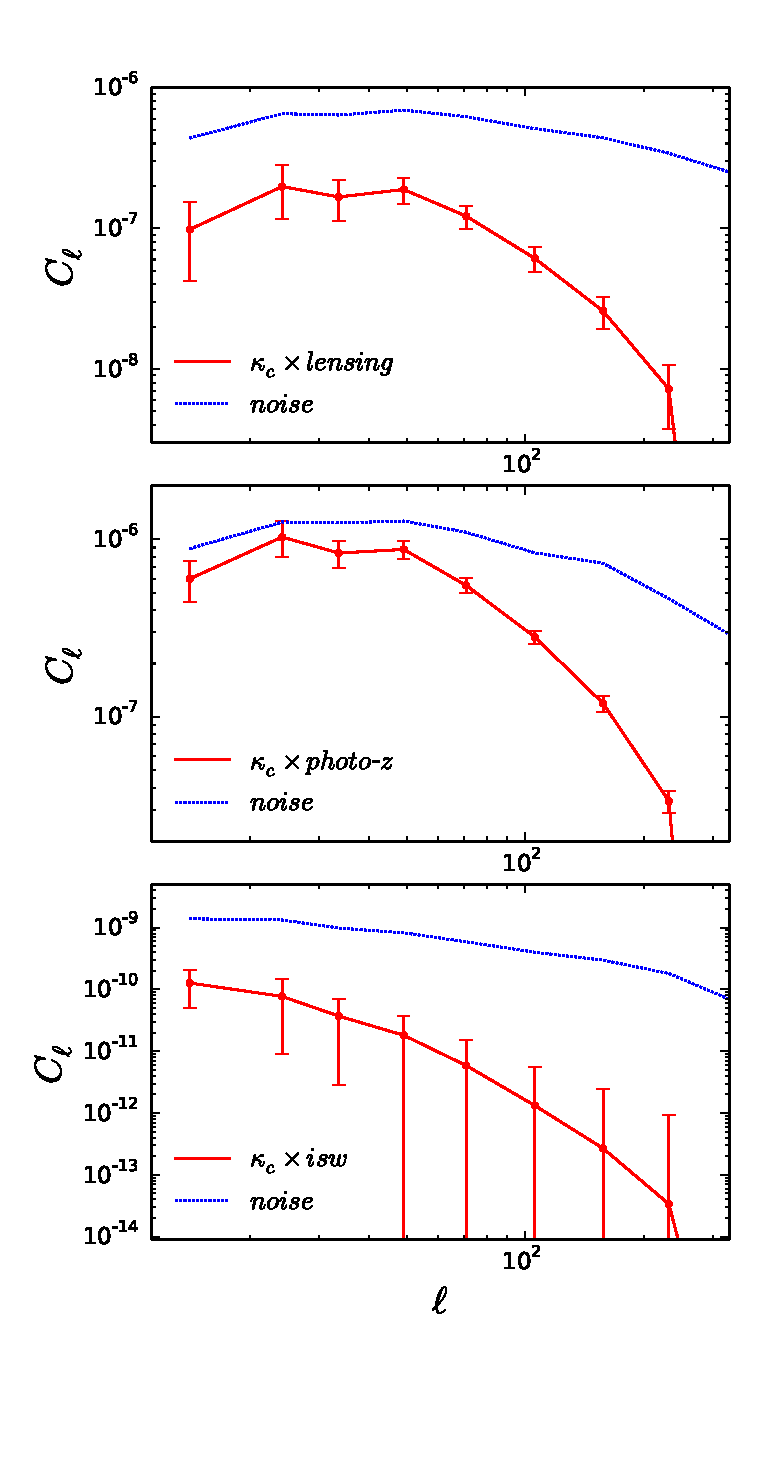
\includegraphics[width=0.48\textwidth]{f8.eps}
%\end{center}
%\vspace{-0.7cm}
%\caption{The cross correlation signals between 21cm and other cosmic probes.}
%\end{figure}

(1) CMB lensing.---The weak lensing convergence is a weighted projection
of the dark matter density fluctuations along the line of sight to the last 
scattering surface,
\begin{eqnarray}
\kappa(\bm{\theta})=\int_0^{\chi_s}d\chi 
W_\kappa(\chi)\delta(\chi\bm{\theta},\chi)\ ,
\end{eqnarray}
where the lensing kernel
\begin{eqnarray}
W_\kappa(\chi)=\frac{3\Omega_{m0}H_0^2\chi(\chi_s-\chi)}{2a(\chi)\chi_s}\ ,
\end{eqnarray}
with $\chi_s=\chi(z_s=1090)$.
To generate the convergence field from simulation data, we first squeeze the 
simulation box to a 2D plane, then multiply the $W(\chi(z=1))$, as the 
lensing weight is a slowly varying function for the case of CMB lensing.
Then we obtain the lensing convergence field contributed by the simulated 
density field.

(2) Photo-$z$ galaxies.---We calculate the projected galaxy density field at 
$z\sim 1$ with usual photo-$z$ bin width of $0.2$, i.e., $z_\mr{p}\in(0.9,1.1)$.
We adopt the galaxy distribution characterized by 
$n(z)\propto z^{\alpha}\mr{exp}[-(z/z^{*})^\beta]$
with $\alpha=2$, $z^*=0.5$, $\beta=1$
and assume the photo-$z$ scatter $\mathcal{P}(z_\mr{p}|z)$ is perfectly known to be in a Gaussian form with photo-$z$ error $\sigma_z=0.05(1+z)$.
The 2D angular galaxy distribution is given by
\begin{eqnarray}
\delta_\mr{2D}(\bm{\theta})=\int_0^\infty dzW_\mr{p}(z)
\delta(\chi(z)\bm{\theta},\chi(z))\ ,
\end{eqnarray}
where the window function 
\begin{eqnarray}
W_\mr{p}(z)\propto\int_{0.9}^{1.1} n(z) \mathcal{P}(z_\mr{p}|z) dz_\mr{p}\ 
\end{eqnarray}
with normalization $\int W_\mr{p}(z)dz=1$.

(3) ISW effect.---The fractional CMB temperature fluctuations induced by the 
ISW effect is given as 
\begin{eqnarray}
\bigg(\frac{\Delta T}{T}\bigg)_\mr{ISW}(\bm\theta)=-2\int_0^{\chi_s}d\chi
\frac{\partial\Phi(\chi\bm{\theta},\chi)}{\partial\chi}\ .
\end{eqnarray}
In Fourier space, approximating that the evolution of $\delta(\bm{k},t)$ with 
time is given by linear theory
$\dot\delta(\bm{k},t)=\dot D(t)\delta(\bm{k},t=0)$, we have
\begin{eqnarray}
\frac{\partial\Phi(\bm{k},\chi)}{\partial\chi}=-\frac{3\Omega_{m0}H_0^2}
{2a(\chi)}\frac{\partial\mr{ln}(D/a)}{\partial\chi}
\frac{\delta(\bm{k},\chi)}{k^2}\ ,
\end{eqnarray}
where $D$ is the growth factor.
In our implementation, we also approximate the time dependent factor as a 
constant across the simulation box.

\begin{figure}[tbp]
\begin{center}
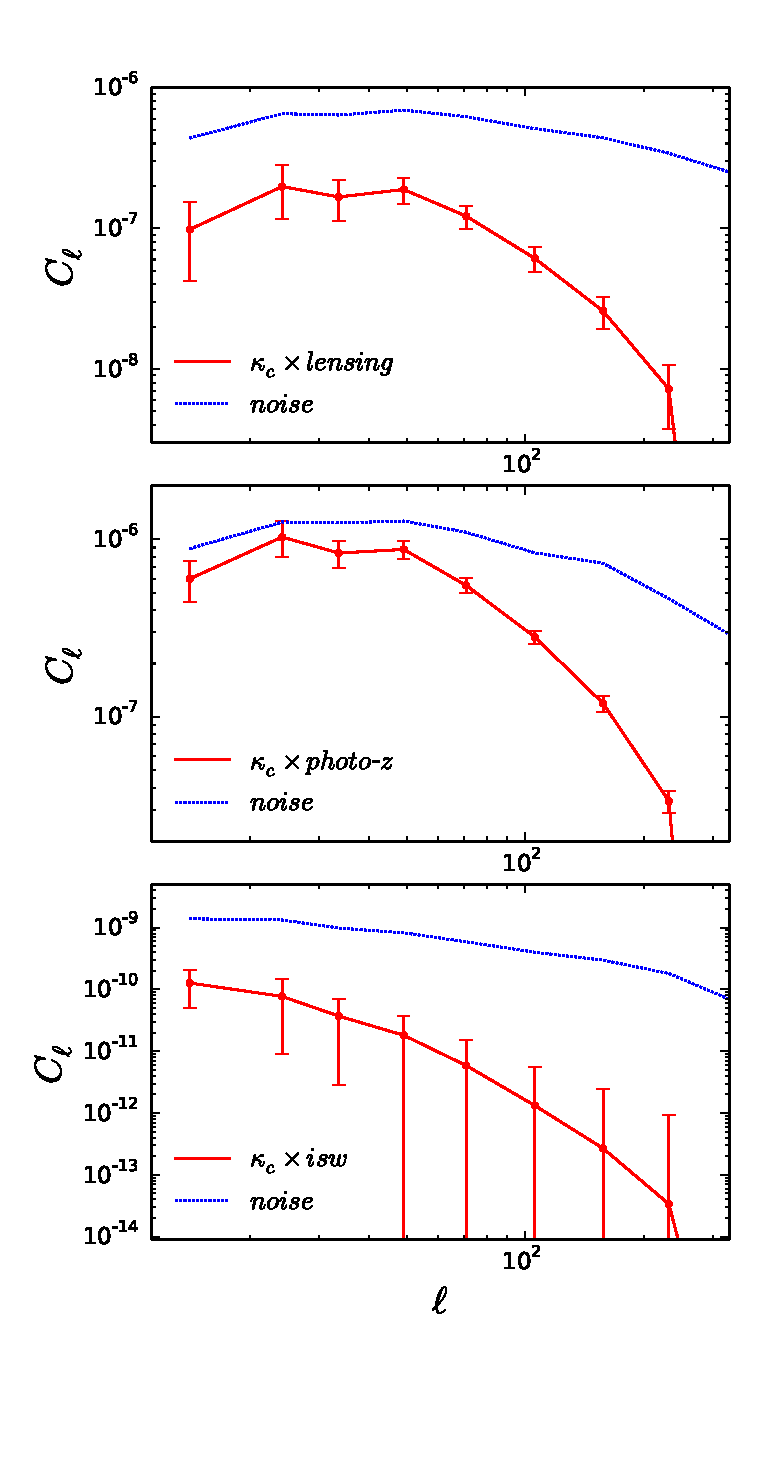
\includegraphics[width=0.48\textwidth]{f8.eps}
\end{center}
\vspace{-1.9cm}
\caption{(Top) The cross correlation of 21 cm and CMB lensing.
(Middle) The correlation of 21 cm and photo-$z$ galaxies. (Bottom) The
correlation of 21 cm and ISW effect. The solid curve shows the signal and the 
dotted curve shows the noise per mode. The results are 
for $R_\parallel=60\ \mr{Mpc}/h$ and $k_c=0.5\ h/\mr{Mpc}$.}
\label{fig:cs}
\end{figure}

In Fig. \ref{fig:cc}, we show the cross-correlation coefficients of 21 cm with 
different observations for both $R_\parallel=60\ \mr{Mpc}/h$ and 
$15\ \mr{Mpc}/h$. Due to the similar treatments of CMB lensing field
and the ISW field, we get the same correlation coefficient for them. 
The correlation with photo-$z$ galaxies is smaller than the other
two since we only use a narrow bin which locates at $z=1$ with bin width $0.2$.

In each panel of Fig. \ref{fig:cs}, we show the cross-correlation signal 
$C_\ell^{ij}$ and noise per mode
$(C_\ell^in_\ell^j+n_\ell^iC_\ell^j+n^i_\ell n^j_\ell)^{1/2}$, where $n_\ell^i$
is the noise power spectrum. The error of the signal is 
\begin{eqnarray}
(\Delta C_\ell^{ij})^2=\frac{1}{(2\ell+1)f_\mr{sky}\Delta\ell}
\bigg[{(C_\ell^{ij})^2+(C_\ell^{i}+n_\ell^{i})
(C_\ell^{j}+n_\ell^{j})}\bigg].
\end{eqnarray}
For the 21 cm field, $n_\ell^\mr{21cm}$ is given through Eq. (\ref{eq:kapc}). 
The noise for CMB lensing is assumed to be the same as Planck 2015 results 
\cite{2015:plancklensing}. For photo-$z$ galaxies, the shot noise is negligible
on degree scales. For ISW effect, $n_\ell^\mr{ISW}$ is the large-scale
CMB power spectrum $C_\ell^{TT}$. We choose $f_\mr{sky}$ to be $0.25$ for 
CMB lensing and photo-$z$ galaxies, and $1$ for the ISW effect. By
using cosmic tidal reconsruction, we are able to detect the cross-correlation
signals with ongoing 21 cm experiments \cite{2014SPIE.9145E..22B,2015ApJ...798...40X,HIRAX}. 
The redshift information contained in 21 cm observations allows us to constrain
the expansion history of the Universe by cross correlating with the ISW effect.
The detectability for ISW effect can be further improved by including CMB 
polarization data \cite{2011PhRvD..83f3001L}.

{\it Discussion.}---It may seem to be odd that the modes lost appear again
after reconstruction. This can be understood intuitively.
The reconstructed field $\kappa_c$ is given by the linear combination of 
quadratic estimators, in the form of 
$\kappa_c(\bm{x})\sim\delta_{fs}(\bm{x})\delta_{fs}(\bm{x})$. In Fourier 
space this can be written as $\kappa_c(\bm{k})\sim\int d^3k'
\delta_{fs}(\bm{k}')\delta_{fs}(\bm{k}-\bm{k}')$, i.e., the reconstructed 
field is given by the convolution of $\delta_{fs}(\bm{k}')$ and 
$\delta_{fs}(\bm{k}-\bm{k}')$. Although $\delta_{fs}$ has no small radial
modes, i.e. $k_{\parallel}'$ and $k_\parallel-k_{\parallel}'$ can not be small,
$k_\parallel$ can reach the low $k_\parallel$ regime.
Here, we extract the information about matter distribution on large scales 
contained in the small-scale matter distributions. The power spectrum of 
$\kappa_c$ is given by the connected four point function of $\delta_{fs}$,
which means we are using the information that comes from higher order statistics
and is not included in the two point statistics of $\delta_{fs}$, i.e., 
power spectrum.

The tidal shear estimators we used are optimal for Gaussian sources and in the 
long-wavelength limit \cite{2015:zhu}.
The results can still be improved by constructing optimal tidal shear 
estimators for non-Gaussian sources as in 21 cm lensing \cite{2010:lu} and 
constructing optimal estimators on all scales. 
This means here we present the ``least optimal'' case of recovering the 
cross-correlation signals and even better results can be achieved in future.

The BAO reconstruction technique \cite{2007:bao} has been shown to be still
useful in 21 cm surveys \cite{2015:bao1,2015:bao2}. While there are not 
many modes with small $k_\parallel$ lost in the foreground subtraction, the 
differential motions which smear the BAO peaks are substantially contributed
by large-scale modes with $k\lesssim0.1\ h/\mr{Mpc}$ \cite{2007:bao}.
The tidal reconstruction compensates the foreground wedge at low $k_\parallel$
and high $k_\perp$ and hence can further improve the BAO reconstruction in 21 cm
surveys. 
%Since all cosmological 21 cm experiments share the same foreground
%problem, no matter low redshift surveys for BAO or high redshift observations
%for the EOR signal, the tidal reconstruction can also help high redshift 
%cross-correlations like the 21 cm-kSZ signal from EOR \cite{2015:marcelo}. 
All 21 cm experiments, no matter the low redshift experiments for BAO effect
or the high redshift experiments for EOR signal, share the same foreground 
problem. Although not examed here, we expect great help from the cosmic tidal
reconstruction in high redshift cross correlations, like 21 cm-kSZ signal from 
EOR \cite{2015:marcelo}.
Based on above discussions, we conclude that cosmic tidal reconstruction is 
extremely valuable for all cosmological 21 cm surveys as well as CMB and
photometric redshift observations.

We acknowledge helpful discussions with Alex van Engelen, Marcelo Alvarez,
Philippe Berger, Yi-Chao Li and Shifan Zuo.
The simulations were performed on the BGQ supercomputer 
at the SciNet HPC Consortium.
SciNet is funded by: the Canada Foundation for Innovation under the auspices 
of Compute Canada;
the Government of Ontario; the Ontario Research Fund -- Research Excellence;
and the University of Toronto.
We acknowledge the support of the Chinese MoST 863 program under Grant 
No. 2012AA121701, the CAS Science Strategic Priority Research Program 
XDB09000000, the NSFC under Grant No. 11373030 and 11403071, IAS at 
Tsinghua University, CHEP at Peking University, and NSERC.
Research at the Perimeter Institute is supported by the Government of Canada 
through Industry Canada and by the Province of Ontario through the Ministry of 
Research $\&$ Innovation.
The Dunlap Institute is funded through an endowment established by the David Dunlap family and the University of Toronto.

\bibliographystyle{apsrev}
\bibliography{cro}

\end{document}
